% Options for packages loaded elsewhere
\PassOptionsToPackage{unicode}{hyperref}
\PassOptionsToPackage{hyphens}{url}
%
\documentclass[
]{report}
\usepackage{amsmath,amssymb}
\usepackage{lmodern}
\usepackage{iftex}
\ifPDFTeX
  \usepackage[T1]{fontenc}
  \usepackage[utf8]{inputenc}
  \usepackage{textcomp} % provide euro and other symbols
\else % if luatex or xetex
  \usepackage{unicode-math}
  \defaultfontfeatures{Scale=MatchLowercase}
  \defaultfontfeatures[\rmfamily]{Ligatures=TeX,Scale=1}
\fi
% Use upquote if available, for straight quotes in verbatim environments
\IfFileExists{upquote.sty}{\usepackage{upquote}}{}
\IfFileExists{microtype.sty}{% use microtype if available
  \usepackage[]{microtype}
  \UseMicrotypeSet[protrusion]{basicmath} % disable protrusion for tt fonts
}{}
\makeatletter
\@ifundefined{KOMAClassName}{% if non-KOMA class
  \IfFileExists{parskip.sty}{%
    \usepackage{parskip}
  }{% else
    \setlength{\parindent}{0pt}
    \setlength{\parskip}{6pt plus 2pt minus 1pt}}
}{% if KOMA class
  \KOMAoptions{parskip=half}}
\makeatother
\usepackage{xcolor}
\IfFileExists{xurl.sty}{\usepackage{xurl}}{} % add URL line breaks if available
\IfFileExists{bookmark.sty}{\usepackage{bookmark}}{\usepackage{hyperref}}
\hypersetup{
  pdftitle={Data Support for Swedish Pharmacy Residents},
  pdfauthor={Jack B. Huber, Ph.D.},
  hidelinks,
  pdfcreator={LaTeX via pandoc}}
\urlstyle{same} % disable monospaced font for URLs
\usepackage{graphicx}
\makeatletter
\def\maxwidth{\ifdim\Gin@nat@width>\linewidth\linewidth\else\Gin@nat@width\fi}
\def\maxheight{\ifdim\Gin@nat@height>\textheight\textheight\else\Gin@nat@height\fi}
\makeatother
% Scale images if necessary, so that they will not overflow the page
% margins by default, and it is still possible to overwrite the defaults
% using explicit options in \includegraphics[width, height, ...]{}
\setkeys{Gin}{width=\maxwidth,height=\maxheight,keepaspectratio}
% Set default figure placement to htbp
\makeatletter
\def\fps@figure{htbp}
\makeatother
\setlength{\emergencystretch}{3em} % prevent overfull lines
\providecommand{\tightlist}{%
  \setlength{\itemsep}{0pt}\setlength{\parskip}{0pt}}
\setcounter{secnumdepth}{-\maxdimen} % remove section numbering
\usepackage{booktabs}
\ifLuaTeX
  \usepackage{selnolig}  % disable illegal ligatures
\fi
\usepackage[]{natbib}
\bibliographystyle{plainnat}

\title{Data Support for Swedish Pharmacy Residents}
\author{Jack B. Huber, Ph.D.}
\date{May 2022}

\begin{document}
\maketitle

\hypertarget{purpose-of-this-document}{%
\chapter{Purpose of this Document}\label{purpose-of-this-document}}

The purpose of this document is to assemble some advice and resources to
support Swedish Pharmacy residents in their journey from project
proposal to a completed research project.

\hypertarget{planning-your-project}{%
\chapter{Planning your Project}\label{planning-your-project}}

\hypertarget{the-causal-logic-of-your-project}{%
\section{The causal logic of your
project}\label{the-causal-logic-of-your-project}}

Fundamentally, the resident research project is an effort to gather
causal evidence for the claim that a particular treatment or way of
utilizing medicine ``worked'' by being more effective than a rival or
pre-existing treatment. To plan data collection for the strongest causal
evidence is the purpose of research design \citep{CampbellStanley1963}.

The ideal research design would be a pure experiment with random
assignment. The resident would randomly assign patients to treatment and
control conditions, then compare outcomes following treatment. In such a
scenario the resident could attribute any significant difference in
outcomes to the treatment because the groups would differ only by chance
in all other ways. Any pre-existing differences would be statistically
insignificant.

Because the resident cannot randomly assign patients to conditions going
forward, the project falls under the category of
\emph{\textbf{quasi-experiment}}. This means it is more vulnerable to
confounding explanations of any difference in outcomes.

The resident research project will culminate in a comparison between two
groups: a pre-implementation group and a post-implementation group. One
difference between the groups is time, and recent history has made a big
difference. Compare a pre-implementation group from the onset of the
pandemic with a high incidence of COVID-19 to a more recent
post-implementation group with much lower incidence of the virus. This
difference between the two groups in COVID-19 infection may combine with
the difference in drug dosing to influence treatment outcomes. This
difference in COVID-19 infection could therefore be a
\emph{\textbf{confound}}.

The point is to clarify:

\begin{itemize}
\tightlist
\item
  What is the outcome to improve? This is the dependent variable.
\item
  What is the difference in treatment intended to cause the improvement
  in the post-implementation group? This is the independent variable.
\item
  All other variables are control variables. They should differ only by
  chance. If there is a noticeable pre-existing difference, and the
  level of that factor in one group affects the outcome, it is a
  confound.
\end{itemize}

\hypertarget{how-many-patients}{%
\section{How many patients?}\label{how-many-patients}}

Possibly the most pressing question for resident research projects is:
How many patients do I need? The resident research project will
culiminate in a series of comparisons between the pre-implementation and
post-implementation groups. Outcomes of the two samples will differ by
at least some quantity. The resident researcher expresses this
difference as an effect, like this:

Assume that this effect suggests more favorable outcomes for the
post-implementation group. This effect raises several questions:

\begin{itemize}
\tightlist
\item
  How do we evaluate this effect?
\item
  Could we attribute it to chance? (because it would be very unlikely
  for both groups to have exactly the same outcomes)
\item
  Or is it larger than that?
\end{itemize}

In statistical terms, this is a question of \textbf{statistical power}.
Power is the ability to isolate a treatment effect when it really does
exist \citep{Cohen1988}. Power is a function of effect size, sample
size, and statistical significance. In order to decide on a number of
patients we need to have a sense of what size of effect we want to
reliably detect.

\begin{figure}
\centering
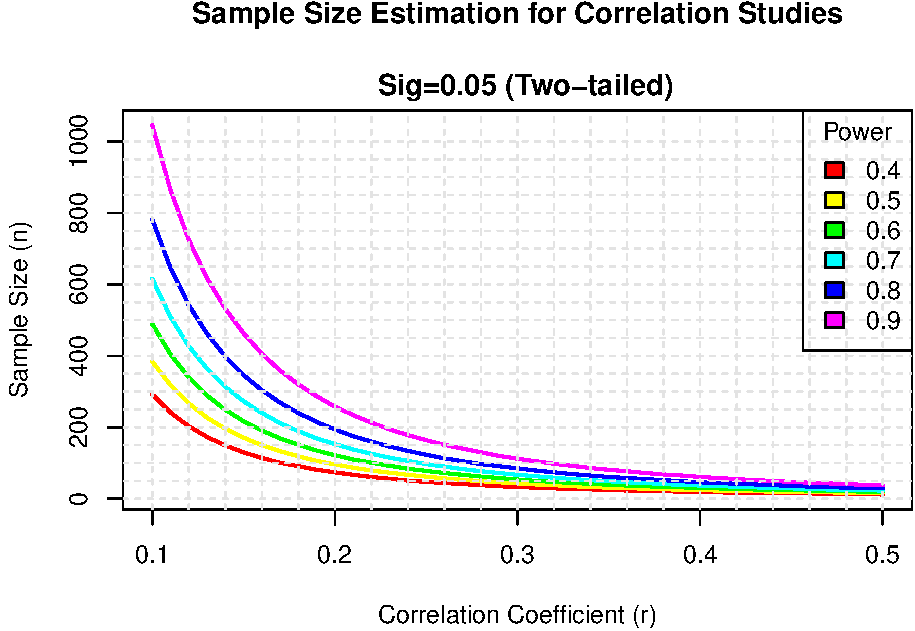
\includegraphics{index_files/figure-latex/power-1.pdf}
\caption{Power Analysis}
\end{figure}

Power is a function of sample size, effect size, and statistical
significance. Figure @ref(fig:power) is a plot of power rates against
these other variables. A large effect (r \textasciitilde{} 0.5) is
detectable with a sample of any size. But only large samples have the
power to detect a statistically significant (p \textless{} .05) small
correlation (r = 0.1).

\hypertarget{collecting-your-data}{%
\chapter{Collecting your Data}\label{collecting-your-data}}

\hypertarget{data-sources}{%
\section{Data Sources}\label{data-sources}}

\begin{itemize}
\tightlist
\item
  Epic
\item
  Cogito dashboards
\item
  SlicerDicer
\item
  Custom reporting (SQL)
\end{itemize}

\hypertarget{granularity}{%
\section{Granularity}\label{granularity}}

\begin{itemize}
\tightlist
\item
  Patient-level data
\item
  Encounter level data
\item
  Medication administration level data
\item
  Lab results level data
\end{itemize}

\hypertarget{advice-for-data-collection}{%
\section{Advice for Data Collection}\label{advice-for-data-collection}}

\begin{enumerate}
\def\labelenumi{\arabic{enumi}.}
\item
  Define the most critical variables.
\item
  Study an exemplar (provided).
\item
  We need to figure out version control. Data proliferation and
  overload.
\end{enumerate}

\hypertarget{analyzing-your-data}{%
\chapter{Analyzing your Data}\label{analyzing-your-data}}

You have data. Congratulations! Let's analyze!

\hypertarget{preparing-your-data-for-analysis}{%
\section{Preparing your data for
analysis}\label{preparing-your-data-for-analysis}}

The first step is to complete a number of tasks to prepare your data for
analysis. One data matrix. See the exemplar.

\hypertarget{choosing-appropriate-statistics}{%
\section{Choosing appropriate
statistics}\label{choosing-appropriate-statistics}}

It is important to know the measurement level of your variables. How do
you express the outcome by which to compare your pre- and post- samples?
Is it\ldots{}

\begin{itemize}
\tightlist
\item
  Mortality rate (\% surviving)? In such a case you would be comparing
  two proportions.
\item
  ``Time to\ldots{}'' a therapeutic level? In such a case you would be
  comparing two different quantities of time.
\end{itemize}

\hypertarget{odds-ratios}{%
\subsection{Odds ratios}\label{odds-ratios}}

\hypertarget{chi-square-test-of-independence}{%
\subsection{Chi-square test of
independence}\label{chi-square-test-of-independence}}

\hypertarget{two-sample-t-test}{%
\subsection{Two-sample t-test}\label{two-sample-t-test}}

\hypertarget{z-test-of-the-difference-of-proportions}{%
\subsection{Z test of the difference of
proportions}\label{z-test-of-the-difference-of-proportions}}

\hypertarget{cohens-d-effect-size}{%
\subsection{\texorpdfstring{Cohen's \emph{d} effect
size}{Cohen's d effect size}}\label{cohens-d-effect-size}}

\hypertarget{reporting-your-results}{%
\chapter{Reporting your Results}\label{reporting-your-results}}

\hypertarget{advice-on-graphs}{%
\section{Advice on graphs}\label{advice-on-graphs}}

\hypertarget{advice-on-tables}{%
\section{Advice on tables}\label{advice-on-tables}}

  \bibliography{bibfile.bib,packages.bib}

\end{document}
